\documentclass[utf8]{earlywinter}
%\usetheme{Dresden}
%\usecolortheme{beaver}
\usepackage[T1]{fontenc}
\usepackage[frenchb]{babel}
\usepackage{graphicx}
\usepackage{hyperref}
\usepackage{amsmath}
\usepackage{mathtools}

\setbeamertemplate{navigation symbols}{}%remove navigation symbols

\defbeamertemplate*{headline}{miniframes theme no subsection}
{%
  \begin{beamercolorbox}[colsep=1.5pt]{upper separation line head}
  \end{beamercolorbox}
  \begin{beamercolorbox}{section in head/foot}
    \vskip2pt\insertnavigation{\paperwidth}\vskip2pt
  \end{beamercolorbox}%
  \begin{beamercolorbox}[colsep=1.5pt]{lower separation line head}
  \end{beamercolorbox}
}

\setbeamertemplate{footline}[miniframes theme no subsection]


\title{Voting Systems}
\author{Aur\`ele Barri\`ere \& Sol\`ene Mirliaz}
\date{04/04/2017}

\begin{document}

\begin{frame}
\maketitle
\end{frame}

\section{Existing systems}
\begin{frame}{\secname}
  US elections:
  \begin{itemize}
    \item Two candidates poorly appreciated
    \item Misrepresentation of the peoples by the Electoral college
  \end{itemize}
  \begin{center}
    
\includegraphics[width=\linewidth]{us.png}
  \end{center}
  
\end{frame}

\section{Examples of voting systems}
\begin{frame}{\secname}
  \framesubtitle{Our example}
  \centering
  \begin{tabular}{r | c c c c c |}
       & A & B & C & D & E \\ \hline
    32 & 1 & 5 & 4 & 2 & 3 \\
    21 & 5 & 1 & 4 & 3 & 2 \\
    17 & 5 & 2 & 1 & 4 & 3 \\
    16 & 5 & 4 & 2 & 1 & 3 \\
    9  & 5 & 2 & 4 & 3 & 1 \\
    3  & 5 & 4 & 2 & 3 & 1 \\ \hline
  \end{tabular}
  \vfill
\end{frame}

\begin{frame}{\secname}
  \framesubtitle{Majority}
  \centering
  \begin{tabular}{r | >{\columncolor{orange!20!white}}c c c c c |}
       & A & B & C & D & E \\ \hline
    \rowcolor{orange!20!white}
    32 & {\bf \color{orange} 1} & 5 & 4 & 2 & 3 \\
    21 & 5 & 1 & 4 & 3 & 2 \\
    17 & 5 & 2 & 1 & 4 & 3 \\
    16 & 5 & 4 & 2 & 1 & 3 \\
    9  & 5 & 2 & 4 & 3 & 1 \\
    3  & 5 & 4 & 2 & 3 & 1 \\ \hline
  \end{tabular}
  
  \vfill
  \begin{tabular}{c c c c c}
  Majority & & & & \\
  A & & & &
  \end{tabular}
\end{frame}

\begin{frame}{\secname}
  \framesubtitle{Two turns}
  \centering
  \begin{tabular}{r | c >{\columncolor{orange!20!white}}c c c c |}
       & A & B & C & D & E \\ \hline
    \rowcolor{orange!20!white}
    32 & 1 & 5 & 4 & 2 & 3 \\
    \rowcolor{orange!20!white}
    21 & 5 & 1 & 4 & 3 & 2 \\
    17 & 5 & 2 & 1 & 4 & 3 \\
    16 & 5 & 4 & 2 & 1 & 3 \\
    9  & 5 & 2 & 4 & 3 & 1 \\
    3  & 5 & 4 & 2 & 3 & 1 \\ \hline
       &32 &{\bf \color{orange} 66} & & &
  \end{tabular}
  
  \vfill
  \begin{tabular}{c c c c c}
  Majority & Two turns & & & \\
  A & B & & &
  \end{tabular}
\end{frame}

\begin{frame}{\secname}
  \framesubtitle{Elimination}
  \centering
  \begin{tabular}{r | c c c c >{\columncolor{red!20!white}}c |}
       & A & B & C & D & E \\ \hline
    32 & 1 & 5 & 4 & 2 & 3 \\
    21 & 5 & 1 & 4 & 3 & 2 \\
    17 & 5 & 2 & 1 & 4 & 3 \\
    16 & 5 & 4 & 2 & 1 & 3 \\
    9  & 5 & 2 & 4 & 3 & 1 \\
    3  & 5 & 4 & 2 & 3 & 1 \\ \hline
       &32 & 21 & 17 &16 &{\bf \color{red} 12}
  \end{tabular}
  
  \vfill
  \begin{tabular}{c c c c c}
  Majority & Two turns & & & \\
  A & B & & &
  \end{tabular}
\end{frame}

\begin{frame}{\secname}
  \framesubtitle{Elimination}
  \centering
  \begin{tabular}{r | c c c c |}
       & A & B & C & D \\ \hline
    32 & 1 & 5 & 4 & 2 \\
    21 & 5 & 1 & 4 & 3 \\
    17 & 5 & 2 & 1 & 4 \\
    16 & 5 & 4 & 2 & 1 \\
    9  & 5 & 2 & 4 & 3 \\
    3  & 5 & 4 & 2 & 3 \\ \hline
       & - & - & - & -
  \end{tabular}
  
  \vfill
  \begin{tabular}{c c c c c}
  Majority & Two turns & & & \\
  A & B & & &
  \end{tabular}
\end{frame}
\begin{frame}{\secname}
  \framesubtitle{Elimination}
  \centering
  \begin{tabular}{r | c c c c |}
       & A & B & C & D \\ \hline
    32 & 1 & 4 & 3 & 2 \\
    21 & 4 & 1 & 3 & 2 \\
    17 & 4 & 2 & 1 & 3 \\
    16 & 4 & 3 & 2 & 1 \\
    9  & 4 & 1 & 3 & 2 \\
    3  & 4 & 3 & 1 & 2 \\ \hline
       & - & - & - & -
  \end{tabular}
  
  \vfill
  \begin{tabular}{c c c c c}
  Majority & Two turns & & & \\
  A & B & & &
  \end{tabular}
\end{frame}
\begin{frame}{\secname}
  \framesubtitle{Elimination}
  \centering
  \begin{tabular}{r | c c c >{\columncolor{red!20!white}}c |}
       & A & B & C & D \\ \hline
    32 & 1 & 4 & 3 & 2 \\
    21 & 4 & 1 & 3 & 2 \\
    17 & 4 & 2 & 1 & 3 \\
    16 & 4 & 3 & 2 & 1 \\
    9  & 4 & 1 & 3 & 2 \\
    3  & 4 & 3 & 1 & 2 \\ \hline
       &32 &30 &20 &{\bf \color{red} 16}
  \end{tabular}
  
  \vfill
  \begin{tabular}{c c c c c}
  Majority & Two turns & & & \\
  A & B & & &
  \end{tabular}
\end{frame}
\begin{frame}{\secname}
  \framesubtitle{Elimination}
  \centering
  \begin{tabular}{r | c >{\columncolor{red!20!white}}c c |}
       & A & B & C \\ \hline
    32 & 1 & 3 & 2 \\
    21 & 3 & 1 & 2 \\
    17 & 3 & 2 & 1 \\
    16 & 3 & 2 & 1 \\
    9  & 3 & 1 & 2 \\
    3  & 3 & 2 & 1 \\ \hline
       & 32 & {\bf \color{red} 30} & 36
  \end{tabular}
  
  \vfill
  \begin{tabular}{c c c c c}
  Majority & Two turns & & & \\
  A & B & & &
  \end{tabular}
\end{frame}
\begin{frame}{\secname}
  \framesubtitle{Elimination}
  \centering
  \begin{tabular}{r | >{\columncolor{red!20!white}}c c |}
       & A & C \\ \hline
    32 & 1 & 2 \\
    21 & 2 & 1 \\
    17 & 2 & 1 \\
    16 & 2 & 1 \\
    9  & 2 & 1 \\
    3  & 2 & 1 \\ \hline
       &{\bf \color{red} 32} &66
  \end{tabular}
  
  \vfill
  \begin{tabular}{c c c c c}
  Majority & Two turns & & & \\
  A & B & & &
  \end{tabular}
\end{frame}
\begin{frame}{\secname}
  \framesubtitle{Elimination}
  \centering
  \begin{tabular}{r | >{\columncolor{orange!20!white}}c |}
       & C \\ \hline
    32 & 2 \\
    21 & 1 \\
    17 & 1 \\
    16 & 1 \\
    9  & 1 \\
    3  & 1 \\ \hline
  \end{tabular}
  
  \vfill
  \begin{tabular}{c c c c c}
  Majority & Two turns & Elimination & & \\
  A & B & C & &
  \end{tabular}
\end{frame}

\begin{frame}{\secname}
  \framesubtitle{Points}
  \centering
  \begin{minipage}[l]{0.3\linewidth}
    \begin{block}{Points}
      \begin{itemize}
        \item 1st $\to$ 5pt
        \item 2nd $\to$ 4pt
        \item 3rd $\to$ 3pt
        \item 4th $\to$ 2pt
        \item 5th $\to$ 1pt
      \end{itemize}
    \end{block}
  \end{minipage}\hspace{20px}
  \begin{minipage}[l]{0.5\linewidth}
    \begin{tabular}{r | c c c >{\columncolor{orange!20!white}}c c |}
         & A & B & C & D & E \\ \hline
      32 & 1 & 5 & 4 & 2 & 3 \\
      21 & 5 & 1 & 4 & 3 & 2 \\
      17 & 5 & 2 & 1 & 4 & 3 \\
      16 & 5 & 4 & 2 & 1 & 3 \\
      9  & 5 & 2 & 4 & 3 & 1 \\
      3  & 5 & 4 & 2 & 3 & 1 \\ \hline
         &226&279&285&{\bf \color{orange}341}&339
    \end{tabular}
  \end{minipage}
  
  \vfill
  \begin{tabular}{c c c c c}
  Majority & Two turns & Elimination & Points & \\
  A & B & C & D &
  \end{tabular}
\end{frame}

\begin{frame}{\secname}
  \framesubtitle{Duel}
  \centering
  \begin{tabular}{r | >{\columncolor{green!20!white}}c c c c >{\columncolor{green!20!white}}c |}
       & A & B & C & D & E \\ \hline
    32 & 1 & 5 & 4 & 2 & 3 \\
    21 & 5 & 1 & 4 & 3 & 2 \\
    18 & 5 & 2 & 1 & 4 & 3 \\
    16 & 5 & 4 & 2 & 1 & 3 \\
    7  & 5 & 2 & 4 & 3 & 1 \\
    3  & 5 & 4 & 2 & 3 & 1 \\ \hline
       & 32 &  &   &   &66
  \end{tabular}
  
  \vfill
  \begin{tabular}{c c c c c}
  Majority & Two turns & Elimination & Points & \\
  A & B & C & D &
  \end{tabular}
\end{frame}

\begin{frame}{\secname}
  \framesubtitle{Duel}
  \centering
  \begin{tabular}{r | c >{\columncolor{green!20!white}}c c c >{\columncolor{green!20!white}}c |}
       & A & B & C & D & E \\ \hline
    32 & 1 & 5 & 4 & 2 & 3 \\
    21 & 5 & 1 & 4 & 3 & 2 \\
    18 & 5 & 2 & 1 & 4 & 3 \\
    16 & 5 & 4 & 2 & 1 & 3 \\
    7  & 5 & 2 & 4 & 3 & 1 \\
    3  & 5 & 4 & 2 & 3 & 1 \\ \hline
       &   &38 &   &   &60
  \end{tabular}
  
  \vfill
  \begin{tabular}{c c c c c}
  Majority & Two turns & Elimination & Points & \\
  A & B & C & D &
  \end{tabular}
\end{frame}

\begin{frame}{\secname}
  \framesubtitle{Duel}
  \centering
  \begin{tabular}{r | c c >{\columncolor{green!20!white}}c c >{\columncolor{green!20!white}}c |}
       & A & B & C & D & E \\ \hline
    32 & 1 & 5 & 4 & 2 & 3 \\
    21 & 5 & 1 & 4 & 3 & 2 \\
    17 & 5 & 2 & 1 & 4 & 3 \\
    16 & 5 & 4 & 2 & 1 & 3 \\
    9  & 5 & 2 & 4 & 3 & 1 \\
    4  & 5 & 4 & 2 & 3 & 1 \\ \hline
       &   &   &33  &   &65
  \end{tabular}
  
  \vfill
  \begin{tabular}{c c c c c}
  Majority & Two turns & Elimination & Points & \\
  A & B & C & D &
  \end{tabular}
\end{frame}
\begin{frame}{\secname}
  \framesubtitle{Duel}
  \centering
  \begin{tabular}{r | c c c >{\columncolor{green!20!white}}c >{\columncolor{green!20!white}}c |}
       & A & B & C & D & E \\ \hline
    32 & 1 & 5 & 4 & 2 & 3 \\
    21 & 5 & 1 & 4 & 3 & 2 \\
    17 & 5 & 2 & 1 & 4 & 3 \\
    16 & 5 & 4 & 2 & 1 & 3 \\
    9  & 5 & 2 & 4 & 3 & 1 \\
    4  & 5 & 4 & 2 & 3 & 1 \\ \hline
       &   &   &   &48 &50
  \end{tabular}
  
  \vfill
  \begin{tabular}{c c c c c}
  Majority & Two turns & Elimination & Points & \\
  A & B & C & D &
  \end{tabular}
\end{frame}
\begin{frame}{\secname}
  \framesubtitle{Duel}
  \centering
  \begin{tabular}{r | c c c c >{\columncolor{orange!20!white}}c |}
       & A & B & C & D & E \\ \hline
    32 & 1 & 5 & 4 & 2 & 3 \\
    21 & 5 & 1 & 4 & 3 & 2 \\
    17 & 5 & 2 & 1 & 4 & 3 \\
    16 & 5 & 4 & 2 & 1 & 3 \\
    9  & 5 & 2 & 4 & 3 & 1 \\
    4  & 5 & 4 & 2 & 3 & 1 \\ \hline
  \end{tabular}
  
  \vfill
  \begin{tabular}{c c c c c}
  Majority & Two turns & Elimination & Points & Duel \\
  A & B & C & D & E
  \end{tabular}
\end{frame}

\begin{frame}{\secname}
  \framesubtitle{Worldwide}
  \centering
    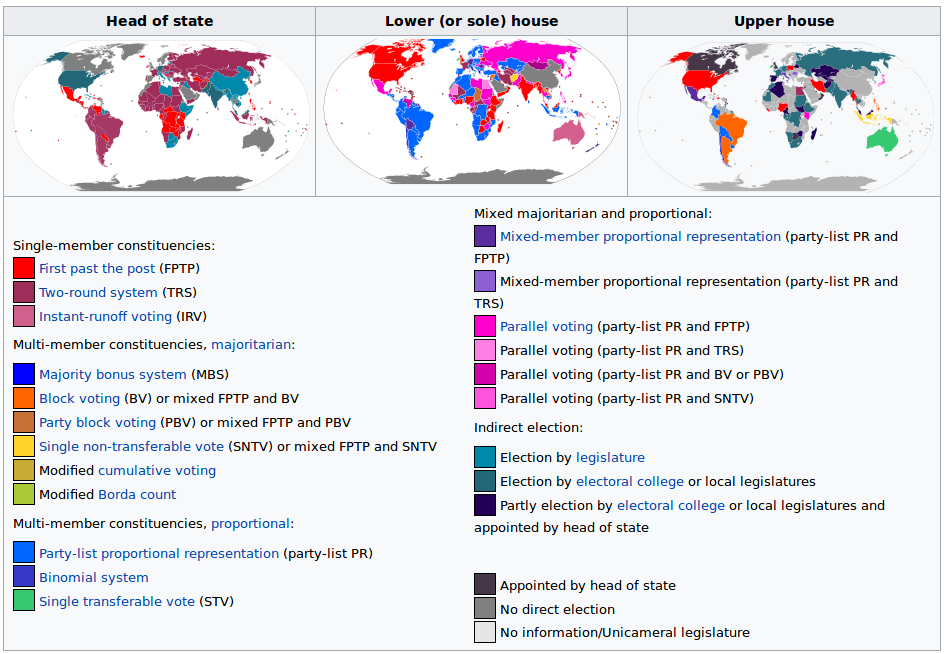
\includegraphics[width=0.9\linewidth]{world.png}
\end{frame}

\section{Social Choice Theory}
\subsection{A formalism for voting systems}
\begin{frame}{\secname: \subsecname}


%  \begin{block}{Social choice setting}
%    \begin{itemize}
%    \item $O$ set of outcomes (or candidates).
%    \item $AGTS$ set of $n$ agents (or voters).
%    \item $L\_ \in L^n$ set of $n$ preference orderings.
%    \end{itemize}
%  \end{block}
%
%
%  \begin{block}{Preference ordering}
%    Total and transitive order on $O$.
%  \end{block}
%
  \begin{block}{Social welfare function}
    %Function $W ~:~(O,AGTS,L\_)\rightarrow L$.
    A voting system is defined as a function. It takes a set of preference orderings and outputs another ordering.
  \end{block}
 

  \begin{minipage}[l]{0.48\linewidth}
    \centering
  \begin{tabular}{r | c c c c c}
       & A & B & C & D & E \\ \hline
    32 & 1 & 5 & 4 & 2 & 3 \\
    21 & 5 & 1 & 4 & 3 & 2 \\
    17 & 5 & 2 & 1 & 4 & 3 \\
    16 & 5 & 4 & 2 & 1 & 3 \\
    9  & 5 & 2 & 4 & 3 & 1 \\
    4  & 5 & 4 & 2 & 3 & 1 \\ 
  \end{tabular}
  \end{minipage}
  \begin{minipage}[r]{0.5\linewidth}
    \centering
    $\xmapsto\qquad A > B > C > D > E$
  \end{minipage}

\end{frame}

\subsection{Interesting Properties}
\begin{frame}{\secname: \subsecname}

  \begin{block}{Pareto efficiency}
    %$\forall o_1,o_2\in O, (\forall i\in AGTS, o_1 >_i o_2) \text{ implies } o_1 >_W o_2$.\\
    {If every voter prefers A to B, then A will also be preferred to B in the result of the vote.}
  \end{block}
  \vfill
  \begin{block}{Independence of Irrelevant Alternatives}
    %$\forall o_1,o_2\in O,\quad\forall >', >''\in L^n,$\\
    %$(\forall i\in AGTS, o_1 >'_i o_2 \text{ iff } o_1 >''_i o_2)\text{ implies }$\\
    %$o_1>_{W(>')} o_2\text{ iff }o_1>_{W(>'')} o_2 $.\\
    {If B lost to A in a first vote, adding a new candidate will not allow B to win over A.}
  \end{block}
\end{frame}


\subsection{Impossibility Theorems}
\begin{frame}{\secname: \subsecname}

  \begin{block}{Arrow's theorem (1970)}
    If the number of candidates is greater or equal than 3, any social welfare function that is Pareto efficient and Independent of irrelevant alternatives is dictatorial.
  \end{block}
  \vfill
  \begin{alertblock}{There won't be a perfect solution.}
  \end{alertblock}

\end{frame}


 
\section[Solutions]{Better voting systems?}

\subsection{ }
\begin{frame}{\secname}

  \begin{exampleblock}{Understanding each voting system}
    Some systems are more biased towards the median (median voter theorem).
  \end{exampleblock}
  \vfill
  \begin{exampleblock}{Choose properties according to the situation}
    What properties are needed for what kind of vote.
  \end{exampleblock}

\end{frame}

\subsection{Other solutions}
\begin{frame}{\subsecname}

  \begin{exampleblock}{Binary Referendums}
    With two issues, plurality voting has every ``good'' property.
  \end{exampleblock}
  \vill
  \begin{exampleblock}{Use technology}
    Voting could be made easier.\\
    Inspiration from voting systems in other contexts (PageRank, approval voting...).
  \end{exampleblock}
  \vill
  \begin{alertblock}{Other issues}
    Some issues does not depend on the voting system.\\
    Abstention, media coverage...
  \end{alertblock}

\end{frame}


\section{Current Research}
\begin{frame}{\secname}

  \begin{itemize}
  \item \url{http://vote.imag.fr/}
  \item \url{https://www.republique-numerique.fr/}
  \item Computer-aided Methods for Social Choice Theory
  \end{itemize}
\end{frame}


\end{document}
